\documentclass[UTF8]{article}

\usepackage{ctex}    %中文环境
\usepackage{datetime}%日期时间
\usepackage{geometry}%调整页边距
\usepackage{pgfplots}%绘制图像
\usepackage{listings}%代码排版
\usepackage{xcolor}   %代码高亮
\usepackage{amsmath} %交叉引用
\usepackage{graphicx}%插入图像
\usepackage[colorlinks,linkcolor=blue]{hyperref}%引用链接

%%%%%%%%%%%%%%%%%%%%%%%%%%%%%%%%定义python代码高亮
\definecolor{dkgreen}{rgb}{0,0.6,0}
\definecolor{gray}{rgb}{0.5,0.5,0.5}
\definecolor{mauve}{rgb}{0.58,0,0.82}


\lstdefinestyle{myPython}{% myPython是格式的名字
	frame=l,
	language=Python,
	aboveskip=3mm,
	belowskip=3mm,
	showstringspaces=false,
	columns=flexible,
	numberstyle=\small\color{red},
	basicstyle={\small\ttfamily},
	keywordstyle=\color{blue},
	commentstyle=\color{dkgreen},
	stringstyle=\color{mauve},
	breaklines=true,
	breakatwhitespace=true,
	tabsize=3
}
%%%%%%%%%%%%%%%%%%%%%%%%%%%%%%%%

%设置页边距
\geometry{left=3cm,right=3.8cm,top=2.5cm,bottom=2.5cm}

\title{\textbf{\huge{基于逻辑回归的分类问题——以鸢尾花分类为例}}}
\author{董明辉 20342006\
(微电子科学与技术学院)}

%%正文
\begin{document}
\maketitle

\newpage
\tableofcontents

\newpage
\section{\textbf{原理}}
\subsection{逻辑回归}
逻辑回归又叫对数几率回归,是一种广义的线性回归分析模型。虽然名字里有回归,但其实是分类模
型,常用于二分类。\par
逻辑回归的原理是用逻辑函数把线性回归结果$(-\infty,\infty)$映射到$(0,1)$。
\subsubsection{线性回归函数}
线性回归函数的数学表达式:
\begin{equation}
	y=\theta_0+\theta_1 x_1+\theta_2 x_2+\cdots+\theta_n x_n=\theta^\mathsf{T} x
	\label{LinearRegression}
\end{equation}
其中$x_i$是自变量,$y$是因变量,$y$的值域为$(-\infty,\infty)$,$\theta_0$是常数项,
$\theta_i(i=1,2,\cdots,n)$是待求系数,不同的权重$\theta_i$反映了自变量对因变量不同的
贡献程度。
\subsubsection{逻辑函数(Sigmoid函数)}
逻辑函数的数学表达式为:
\begin{equation}
	g(z)=\frac{1}{1+e^{-z}}
\end{equation}

逻辑函数的图像为:\par
\begin{tikzpicture}
	\begin{axis}[xlabel=$z$,
			ylabel=$g(z)$,
			title={Sigmoid函数},
			xmin=-10.2,xmax=10.2]
		\addplot[color=blue,domain=-10:10]{1/(1+exp(-x))};
	\end{axis}
\end{tikzpicture}

从Sigmoid函数的图像中我们可以看出当$z$趋于$-\infty$时,$g(z)$趋于0,当$z$趋于$\infty$
时,$g(z)$趋于1,且函数的值域为$(0,1)$,而概率也是介于0到1的数,因此我们可以将Sigmoid
函数的值域与概率联系起来。

\noindent\textbf{逻辑函数的导函数:}\par
逻辑函数的表达式为:
\begin{equation}
	g(y)=\frac{1}{1+e^{-y}}=\frac{e^y}{1+e^y}\label{Sigmoid}
\end{equation}
\par
导函数为:
\begin{equation}
	g'(y)=\frac{e^y(1+e^y)-y*e^y}{(1+e^y)^2}
\end{equation}
\par
经过变换我们可以得到:
\begin{equation}
	g'(y)=g(y)*[1-g(y)]
\end{equation}

\subsubsection{逻辑回归函数}
将线性回归函数的结果$y$,放到Sigmoid函数中去,就构成了逻辑回归函数,即:
\begin{equation}
	g(y)=\frac{1}{1+e^{-y}}	=\frac{1}{1+e^{-(\theta_0+\theta_1 x_1+\cdots+\theta_n x_n)}}
	=\frac{1}{1+e^{-\theta^\mathsf{T}x}} \label{LogisticRegressionFunction}
\end{equation}
\par
以鸢尾花为例,鸢尾花的特征即为\eqref{LogisticRegressionFunction}中的$x$,我们可以
这些样本数据训练逻辑回归模型,求解得到$x$的参数$\theta$。

\subsection{求解逻辑回归中的参数}
\subsubsection{极大似然函数}
以二分类为例,令山鸢尾的标签为0,杂色鸢尾的标签为1,根据\eqref{LogisticRegressionFunction}
得到杂色鸢尾的概率为:
\begin{equation}
	p(Y=1|x)=\frac{1}{1+e^{-\theta^\mathsf{T} x}}
\end{equation}
\par
相应的山鸢尾的概率为:
\begin{equation}
	p(Y=0|x)=1-p(Y=1|x)=1-\frac{1}{1+e^{-\theta^\mathsf{T} x}}=
	\frac{1}{1+e^{\theta^\mathsf{T} x}}
\end{equation}
\par
再令:
\begin{equation}
	\frac{1}{1+e^{-\theta^\mathsf{T} x}}=g(y)=g_\theta (x)
\end{equation}
\par
则杂色鸢尾花的后验概率可写为:
\begin{equation}
	p(Y=1|x)=g_\theta (x)
\end{equation}
\par
山鸢尾的后验概率可写为:
\begin{equation}
	p(Y=0|x)=1-g_\theta (x)
\end{equation}
\par
对于一个鸢尾花的样本数据$(x,y)$,它的标签是y的概率为:
\begin{equation}
	p(y|x;\theta)=(g_\theta (x))^y(1-g_\theta (x))^{1-y}\label{IrisesAPosterioriProbability}
\end{equation}
\par
其中$y\in {0,1}$。当$y=0$时,\eqref{IrisesAPosterioriProbability}表示山鸢尾的概率;
当$y=1$时,表示杂色鸢尾的概率。
\par
当有m个观测样本时,合事件发生的总概率为每个样本发生的概率相乘,即为似然函数,可以写成:
\begin{equation}
	L(\theta)=\prod_{i=1}^{m}p(y_i|x_i;\theta)
	=\prod_{i=1}^{m}(g_\theta (x_i))^{y_i}(1-g_\theta (x_i))^{1-y_i}
\end{equation}
\par
其中$\theta$为待求参数。
\par
为了方便求解,引入不改变函数单调性的对数$\ln$,把连乘变成求和,得到对数似然函数:
\begin{equation}
	l(\theta)=\ln(L(\theta))=\sum_{i=1}^{m}\ln(p(y_i|x_i;\theta))
	=\sum_{i=1}^{m}(y_i\ln(g_\theta (x_i))+(1-y_i)\ln(1-g_\theta (x_i)))
\end{equation}
\par
到这里,我们可以由对数似然函数构造损失函数,用梯度下降法求出使得损失最小的参数$\theta$。
\subsubsection{构造损失函数}
结合逻辑回归中的极大似然函数,取整个数据集上的平均对数似然损失,我们可以得到:
\begin{equation}
	J(\theta)=-\frac{1}{m}\ln(L(\theta)) \label{LossFunction}
\end{equation}
\par
其中$J(\theta)$为损失函数,由对数似然函数前面加负号取平均得到。
\par
因此,在逻辑回归模型中,最大化似然函数和最小化损失函数实际上是等价的,即:
\begin{equation}
	\max \ln(L(\theta))\Leftrightarrow \min J(\theta)
\end{equation}
\par
至此,可由梯度下降法求解得到损失函数最小所对应的参数$\theta$。
\subsubsection{梯度下降法}
梯度下降法的基本思想是:
\begin{enumerate}
	\item 明确现在所处的位置;
	\item 找到该处下降最快的方向,即梯度相反的方向;
	\item 沿着梯度相反方向走一个步长,到达新的位置;
	\item 判断是否梯度为零,如果没有则重复步骤一,否则如果达到则停止。
\end{enumerate}
\par
由损失函数\eqref{LossFunction}可知:
\begin{equation}
	J(\theta)=-\frac{1}{m}\sum_{i=1}^{m}(y_i\ln(g_\theta (x_i))+(1-y_i)\ln(1-g_\theta (x_i)))
\end{equation}
\par
对损失函数求偏导可得:
\begin{equation}
	\frac{\partial J(\theta)}{\partial \theta_j}=
	\frac{1}{m}\sum_{i=1}^{m}[g(\theta^\mathsf{T} x_i)-y_i]*x_i^j
\end{equation}
\par
至此,找到了梯度下降的方向,只要给定一个步长就可以用迭代的方式求解出待求参数$\theta$。

\subsection{利用二分类实现多分类}
利用二分类实现三分类的方法是\textbf{使用多次二分类}。\par
以鸢尾花为例,设山鸢尾的标签为1,其余两种鸢尾花的标签为0,利用样本数据得到一个模型1,
该模型可用来预测测试样本是鸢尾花的概率。同理,再分别令杂色鸢尾,维吉尼亚鸢尾的标签为1,
其余两种鸢尾花标签为0。用同样的样本训练得到模型2,模型3。最后,将测试样本分别通过模型1,
模型2,模型3得到分别是山鸢尾、杂色鸢尾、维吉尼亚鸢尾的概率,最大的概率所对应的就是预测的
该样本的类型。

\section{代码实现}
基于以上原理,可以利用Python来实现以上逻辑回归分类。
\subsection{LogisticRegressionSelf类}
首先,我们先构造一个包含逻辑回归模型的类,类中包括参数$\theta$,训练模型的函数,做出预测的函数。
\par
完整代码见附录。\\
\textbf{导入numpy包:}
\begin{lstlisting}[style=myPython]
import numpy as np
\end{lstlisting}
\textbf{创建类和初始化函数:}
\begin{lstlisting}[style=myPython]
class LogisticRegressionSelf:
	def __init__(self):
		"""初始化LogisticpegressionSelf模型"""
		self.coef_ = None  #维度
		self.intercept_ = None  #截距
		self._theta = None
\end{lstlisting}
\textbf{根据\eqref{Sigmoid}构造Sigmoid函数:}
\begin{lstlisting}[style=myPython]
	def _sigmoid(self, x):
		y = 1.0 / (1.0 + np.exp(-x))
		return y
\end{lstlisting}
\textbf{构造训练模型的函数,包括损失函数$J(\theta)$,损失函数的导数$dJ(\theta)$,模拟梯度下降的函数。}
\begin{lstlisting}[style=myPython]
	def fit(self, X_train, y_train, eta=0.01, n_iters=1e4):
		assert X_train.shape[0] == y_train.shape[0], '训练数据集的长度需要和标签长度保持一致'
		#计算损失函数
		def J(theta, X_b, y):
			p_predcit = self._sigmoid(X_b.dot(theta))
			try:
				return -np.sum(y * np.log(p_predcit) +
							   (1 - y) * np.log(1 - p_predcit)) / len(y)
			except:
				return float('inf')
		#求sigmoid梯度的导数
		def dJ(theta, X_b, y):
			x = self._sigmoid(X_b.dot(theta))
			return X_b.T.dot(x - y) / len(X_b)
		#模拟梯度下降
		def gradient_descent(X_b,y,initial_theta,eta,n_iters=1e4,epsilon=1e-8):
			theta = initial_theta
			i_iter = 0
			while i_iter < n_iters:
				gradient = dJ(theta, X_b, y)
				last_theta = theta
				theta = theta - eta * gradient
				i_iter += 1
				if (abs(J(theta, X_b, y) - J(last_theta, X_b, y)) < epsilon):
					break
			return theta
		X_b = np.hstack([np.ones((len(X_train), 1)), X_train])
		initial_theta = np.zeros(X_b.shape[1])  #列向量
		self._theta = gradient_descent(X_b, y_train, initial_theta, eta,n_iters)
		self.intercept_ = self._theta[0]  #截距
		self.coef_ = self._theta[1:]  #维度
		return self
\end{lstlisting}
\textbf{构造概率预测函数以及根据概率实现二分类的函数:}
\begin{lstlisting}[style=myPython]
	def predict_proba(self, X_predict):
		X_b = np.hstack([np.ones((len(X_predict), 1)), X_predict])
		return self._sigmoid(X_b.dot(self._theta))
	def predict(self, X_predict):
		proba = self.predict_proba(X_predict)
		return np.array(proba > 0.5, dtype='int')
\end{lstlisting}
\subsection{主程序}
上述代码已经构造了逻辑回归需要用到的模型,接下来在主程序中导入逻辑分类所需要的数据,
划分训练集,测试集,并进行数据可视化。\\
\textbf{导入需要用到的包:}
\begin{lstlisting}[style=myPython]
import matplotlib.pyplot as plt#可视化用
import numpy as np
from sklearn.datasets import load_iris#训练和测试所用数据
from LogisticRegressionSelf import LogisticRegressionSelf#逻辑回归类
\end{lstlisting}
\textbf{导入数据:}
\begin{lstlisting}[style=myPython]
iris = load_iris()
\end{lstlisting}
\textbf{对导入的数据进行可视化处理:}
\begin{lstlisting}[style=myPython]
##取100个样本,取前两列特征,花萼长度和宽度
x = iris.data[0:150, 0:2]
y = iris.target[0:150]
##分别取前两类样本,0和1
samples_0 = x[y == 0, :]  #把y=0的样本取出来
samples_1 = x[y == 1, :]
samples_2 = x[y == 2, :]
# 散点图可视化
p1 = plt.scatter(samples_0[:, 0], samples_0[:, 1], marker='o', color='g')
p2 = plt.scatter(samples_1[:, 0], samples_1[:, 1], marker='o', color='r')
p3 = plt.scatter(samples_2[:, 0], samples_2[:, 1], marker='o', color='b')
plt.xlabel(iris.feature_names[0])
plt.ylabel(iris.feature_names[1])
plt.legend([p1, p2, p3], iris.target_names[0:3], loc='upper right')
plt.grid()
\end{lstlisting}
\textbf{得到的图像如下所示:}
\begin{figure}[htbp]
	\centering
	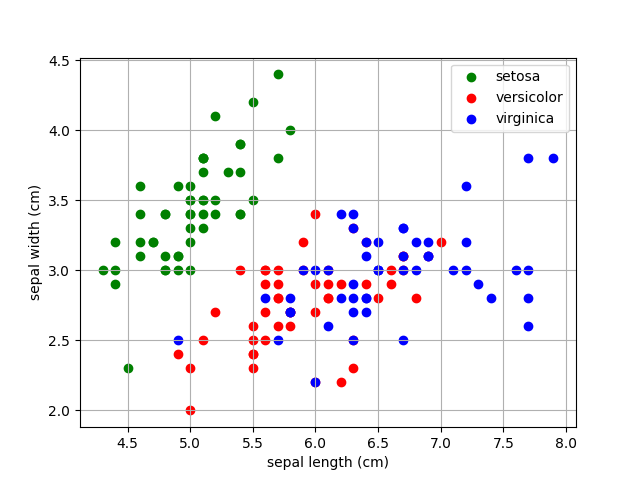
\includegraphics[width=12.0cm,height=9.0cm]{picture/鸢尾花分类_原始数据.png}
	\caption{导入的数据}
\end{figure}

\noindent \textbf{划分测试/训练数据,120个训练数据,30个测试数据:}
\begin{lstlisting}[style=myPython]
x_train = np.vstack([x[:40, :], x[50:90], x[100:140]])
y_train = np.concatenate([y[:40], y[60:100], y[100:140]])
x_test = np.vstack([x[40:50], x[90:100], x[140:]])
y_test = np.concatenate([y[40:50], y[90:100], y[140:]])
\end{lstlisting}
\textbf{训练得到3个模型,分别预测样本为山鸢尾、杂色鸢尾、维吉尼亚鸢尾的概率:}
\begin{lstlisting}[style=myPython]
z_proba = []
lr = []
for i in range(3):
	lr.insert(i, LogisticRegressionSelf())
	lr[i].fit(x_train, np.where(y_train == i, 1, 0),n_iters=1e5)
\end{lstlisting}
\textbf{将样本数据输入到概率预测函数,得到三组概率,取概率最大的为该样本作为该样本的类型:}
\begin{lstlisting}[style=myPython]
for i in range(3):
    z_proba.insert(i, lr[i].predict_proba(x_test))

num_test = x_test.shape[0]
prediction = np.argmax(z_proba, axis=0)#返回每一列最大值的索引
accuracy = np.sum(prediction == y_test) / num_test
print(r'the accuracy of prediction is :', accuracy)
\end{lstlisting}
\textbf{输出为:the accuracy of prediction is : 0.8}\\
\textbf{可视化处理:}
\begin{lstlisting}[style=myPython]
nx, ny = 1000, 500
x_min, x_max = plt.xlim()
y_min, y_max = plt.ylim()
x_grid, y_grid = np.meshgrid(np.linspace(x_min, x_max, nx),
							 np.linspace(y_min, y_max, ny))

for i in range(3):
	z_proba[i] = lr[i].predict_proba(np.c_[x_grid.ravel(), y_grid.ravel()])

z_prediction = np.argmax(z_proba, axis=0)
z_prediction = z_prediction[:].reshape(x_grid.shape)

# plt.contour(x_grid,y_grid,z_prediction,colors=['k'])
plt.contourf(x_grid,y_grid,z_prediction,2,alpha=0.3,colors=['g','r','b'])
plt.show()
\end{lstlisting}

\section{结果}
终端输出为:the accuracy of prediction is : 0.8
\par
分类效果如下图\ref{1}所示
\begin{figure}[htbp]
	\centering
	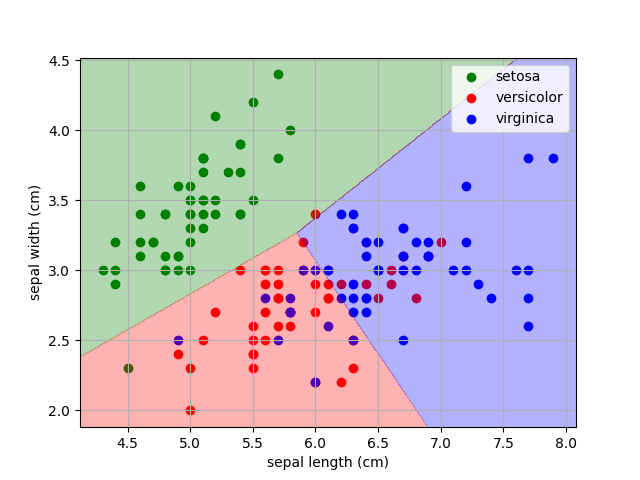
\includegraphics[width=12.0cm,height=9.0cm]{picture/鸢尾花分类.png}
	\caption{鸢尾花逻辑回归分类效果}
	\label{1}
\end{figure}

\section{附录(完整代码)}
\noindent \textbf{LogisticRegressionSelf类代码:}
\lstinputlisting[style=myPython]{code/LogisticRegressionSelf.py}
\textbf{主程序代码:}
\lstinputlisting[style=myPython]{code/main.py}

\end{document}